\documentclass[a4paper]{article} 
\addtolength{\hoffset}{-2.25cm}
\addtolength{\textwidth}{4.5cm}
\addtolength{\voffset}{-3.25cm}
\addtolength{\textheight}{5cm}
\setlength{\parskip}{0pt}
\setlength{\parindent}{0in}

\usepackage[square,sort,comma,numbers]{natbib}
\usepackage{blindtext} % Package to generate dummy text
\usepackage{charter} % Use the Charter font
\usepackage[utf8]{inputenc} % Use UTF-8 encoding
\usepackage{microtype} % Slightly tweak font spacing for aesthetics
\usepackage{amsthm, amsmath, amssymb} % Mathematical typesetting
\usepackage{float} % Improved interface for floating objects
\usepackage{hyperref} % For hyperlinks in the PDF
\usepackage{graphicx, multicol} % Enhanced support for graphics
\usepackage{xcolor} % Driver-independent color extensions
\usepackage{pseudocode} % Environment for specifying algorithms in a natural way
\usepackage[yyyymmdd]{datetime} % Uses YEAR-MONTH-DAY format for dates

\usepackage{fancyhdr} % Headers and footers
\pagestyle{fancy} % All pages have headers and footers
\fancyhead{}\renewcommand{\headrulewidth}{0pt} % Blank out the default header
\fancyfoot[L]{} % Custom footer text
\fancyfoot[C]{} % Custom footer text
\fancyfoot[R]{\thepage} % Custom footer text
\newcommand{\note}[1]{\marginpar{\scriptsize \textcolor{red}{#1}}} % Enables comments in red on margin

%----------------------------------------------------------------------------------------

%\usepackage[maxnames=10]{biblatex}
%-------------------------------
%	TITLE VARIABLES (identify your work!)
%-------------------------------

\usepackage{xcolor}
\usepackage{hyperref}
\usepackage{booktabs}
\usepackage{bbm}

\newcommand{\yourname}{Alex Castilio dos Santos \\Eduardo Alves da Silva \\Joao Felipe Guedes da Silva \\ Leonardo Barreto Alves \\  Maria Gabriella Andrade Felgas \\ Miguel Fernandes de Sousa \\ Pedro Henrique Lopes Leite \\ Renan da Silva Alves \\ Wallace Costa de Abreu \\ Gutemberg Machado Lopes} % replace YOURNAME with your name
%\newcommand{\yournetid}{YOURNETID} % replace YOURNETID with your NetID
\newcommand{\youremail}{guedes.joaofelipe@poli.ufrj.br} % replace YOUREMAIL with your email
\newcommand{\assignmenttitle}{}
\newcommand{\assignmentnumber}{1}

\renewcommand{\thesubsection}{\alph{subsection})}

\begin{document}

%-------------------------------
%	TITLE SECTION (do not modify unless you really need to)
%-------------------------------
\fancyhead[C]{}
\hrule \medskip
\begin{minipage}{0.295\textwidth} 
\raggedright
\footnotesize
\yourname \hfill\\ 
\yournetid \hfill\\ 
\youremail
\end{minipage}
\begin{minipage}{0.4\textwidth} 
\centering 
\large 
CPE793 - Tópicos em Codificação de Áudio - 2021.2\\ 
\normalsize 
Lista \assignmentnumber\\ 
\end{minipage}
\begin{minipage}{0.295\textwidth} 
\raggedleft
\today\hfill\\
\end{minipage}
\medskip\hrule 
\bigskip


%-------------------------------
%	ASSIGNMENT CONTENT (add your responses)
%-------------------------------
\section{Chapter 1}

\subsection{Data rates:}

\begin{enumerate}
    \item $I_1=	8\times10^3\times8\times1=64 \text{ Kbps}$
	\item $I_2=44.1\times10^3\times16\times2=1.4112\text{ Mbps}$
	\item $I_3=44.1\times10^3\times16\times5=3.528 \text{ Mbps}$
	\item $I_4=96\times10^3\times24\times5=11.52 \text{ Mbps}$
\end{enumerate}

\subsection{The need for compression:}

\begin{enumerate}
    \item $	S=11.52\times10^6\times2\times60\times60=82.944 \text{ Gb}$
	\item $	r_{CD}=11.52/1.411\approx8.16$
	\item $	r_{DVD}=11.52/6.144\approx1.87$
\end{enumerate}

\section{Chapter 2}


\subsection{Plotar sobrepostos os gráficos de “$\mu$-law” (com $\mu$ = 255 e b = e) e “A-law” (com A = 87.56).}

Os plots para diferentes valores de $A$ e $\mu$ são apresentados na Figura \ref{fig:companding} para valores de entrada $x$ normalizados entre 0 e 1. Para observar os efeitos da escolha de $A$, incluímos alguns valores adicionais. 

\begin{figure}[h]
    \centering
    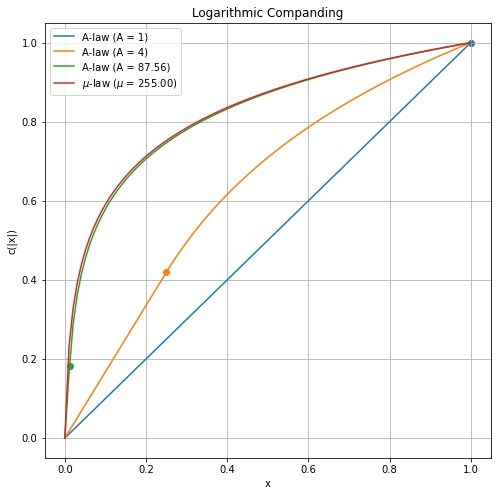
\includegraphics[width=15cm]{images/logaritmic_companding.jpeg}
    \caption{Logarithmic Companding}
    \label{fig:companding}
\end{figure}

Dada a fórmula de compressão da $A$-law na Equação \ref{eq:alaw}

\begin{equation}
  c_A(|x|) =
    \begin{cases}
      \frac{1+\ln (A\cdot |x|)}{1+\ln A}\ \text{if}\ |x| > \frac{1}{A}\\
      \frac{A}{1+\ln A} |x|\ \ \text{otherwise}
    \end{cases}       
    \label{eq:alaw}
\end{equation} vemos que para $|x| \in [0, 1/A]$ a equação é linear e com derivada $d c(|x|)/ d x$ idealmente maior que 1. Isto significa que uma variação pequena no sinal de entrada $x$ será mapeada em uma variação grande no sinal de saída $c(|x|)$, configurando um comportamento de expansão até $x = 1/A$.\\

Por outro lado, para $x > 1/A$ a equação da $A$-law apresenta uma diminuição da derivada conforme a amplitude do sinal de entrada aumenta, fazendo com que o mapeamento diminua a ponto de ficar menor que 1, configurando um comportamento de compressão. \\

Portanto, vemos que a escolha do parâmetro $A$ impacta diretamente em um ponto crítico de operação linear do \textit{companding} logarítmico: quanto maior este parâmetro, maior será a taxa de expansão para sinais de baixa amplitude e compressão para altas amplitudes.

\subsection{Working with bits}

O código com a resolução do exercício 8.2a encontra-se \href{https://github.com/guedes-joaofelipe/CPE793-topics-in-audio-codification/blob/main/exercises/chap02/exercises_chap02.ipynb}{\textit{neste link}}.

%\bibliographystyle{acm}

%\bibliography{references} % citation records are in the references.bib document

\end{document}
